\documentclass{article}
\usepackage{arxiv}
\usepackage[utf8]{inputenc} % allow utf-8 input
\usepackage[T1]{fontenc}    % use 8-bit T1 fonts
\usepackage{hyperref}       % hyperlinks
\usepackage{url}            % simple URL typesetting
\usepackage{booktabs}       % professional-quality tables
\usepackage{amsfonts}       % blackboard math symbols
\usepackage{nicefrac}       % compact symbols for 1/2, etc.
\usepackage{microtype}      % microtypography
\usepackage{lipsum}
\usepackage{graphicx}
\usepackage{subcaption}

\title{A Spatial Analysis of Housing Prices and Neighbourhood Characteristics in London}

\author{
  \large{Kengo Arao}\thanks{With heartfelt thanks to Dr David Candon for dedicated supervision and to Dr Andrei Potlogea for guidance in urban economics}      \thanks{Data and code for this paper are publicly available at \href{https://github.com/KengoA/spatial-analysis-london}{https://github.com/KengoA/spatial-analysis-london}} \\
  Exam Number: B059089 \\
  School of Economics\\
  The University of Edinburgh\\
  \texttt{kengoarao@outlook.com}
}

\begin{document}
\maketitle

\begin{abstract}
\lipsum[1]
\end{abstract}

% keywords can be removed
% \keywords{First keyword \and Second keyword \and More}
\begin{center}
    \textbf{Word Count}: 10,000
\end{center}

\newpage
\tableofcontents

\newpage
\section{Introduction}
 In every metropolitan area, housing price has a strong influence over individual consumption choices and hence important implications in social mobility and quality of life. In light of the rapid urbanisation with 68\% of the world population expected to live in urban areas by 2050 (United Nations, 2018), the underlying mechanism of urban housing markets has been under heavy scrutiny in the fields of urban research and economic geography, while being a focal point of major media outlets in the United Kingdom (The Guardian, 2019; The Independent, 2019).
 
 This paper's empirical analysis builds on the bid-rent theory by Alonso (1964) and integrates the hedonic pricing model by Rosen (1974), where I estimate the coefficients associated with commuting cost to the Central Business District (CBD) and those of urban amenities such as private schools and supermarkets. 
 
 
  One example of dynamically changing urban landscapes is the penetration of German supermarkets into the British grocery market in recent years (Davey, 2018), whose low-price policies likely affect consumption behaviours at a local level. 


This paper provides novelty in two respects. The first is construction of urban amenity variables from OpenStreetMap, an open-sourced collaborative mapping project, which is applicable beyond the scope of the Greater London Area that my empirical analysis of their effects on housing prices is subject to. The second is the application of Rosen's hedonic pricing model (1974) to neighbourhoods instead of individual dwellings, where I utilise two measures of commuting costs and 
establish causality from supermarkets and 



\section{Literature Review and Conceptual Framework}
\subsection{Current Research on Housing Prices}
\subsection{Monocentric City Model}
This paper employs a geographic economic theory by Alonso (1964), Mills (1967) and Muth (1967) called bid-rent theory, which refers to the relationship between the distance from the the city centre and real estate price. The basic intuition is that the housing price increases as you move closer towards the Central Business District (CBD), and consumers face a trade-off between housing costs and commuting costs. A simple version of this model described below underpins the empirical specifications throughout this paper and requires the following five assumptions, the first of which will be relaxed in the next section.
\begin{itemize}
\setlength\itemsep{0.1em}
\item Residents are homogenous and live in a featureless urban area where all the jobs are located in the CBD
\item Each resident is a worker and commutes to a job in the CBD
\item Each worker receives an urban wage $w$ with inelastic labour supply
\item Commuting from distance $d$ entails a linear commuting cost $t(d) = \tau d$
\item Each worker consumes 1 unit of housing which is produced solely  with land
\end{itemize}
Let $p_H (d)$ denote the price of housing located at distance $d$ from the CBD, then a worker's preference can be written as a linear utility function:
\begin{center}
$u = w - p _ { H } ( d ) - t ( d ) = w - p _ { H } ( d ) - \tau d$
\end{center}
With an outside option in the hinterland $\overline{u}$, the spatial equilibrium requires
\begin{center}
$u = w - p _ { H } ( d ) - \tau d = \overline { u }$
\end{center}
Rearranging and partially differentiating $p_H (d)$ with respect to $d$ yields 
\begin{center}
$\frac { \partial p _ { H } ( d ) } { \partial d } = t ^ { \prime } ( d ) = - \tau \quad \forall d \leq \overline { d }$
\end{center}
Let $\overline{d}$ be the upper bound for distance and $\underline{r} > 0$ be the rent for alternative use of land. Then, the equilibrium rent can be written as:

\begin{center}
$p _ { H } ( d ) = \underline { r } + \int _ { d } ^ { \overline { d } } t ^ { \prime } ( \delta ) d \delta = \underline { r } + \tau ( \overline { d } - d )$
\end{center}
Since the alternative land rent $\underline{r}$ is difficult to estimate in practice, I flip the sign of the equation such that 
\begin{center}
$p _ { H } ( d ) = \overline { r } - \int _ { \underline { d } } ^ { d } t ^ { \prime } ( \delta ) d \delta = \overline { r } - \tau ( d - \underline { d } )$
\end{center}
where $\overline{r}$ is the rent in the CBD and $\underline{d}$ is the lower bound for distance, which is 0 at the CBD. This equation hence represents a function of the price of housing which is linearly decreasing in distance from the CBD $d$, which is simply
\begin{center}
$p _ { H } ( d ) = \overline { r } - \tau d$
\end{center}
This will be the basis of the univariate regression models where I estimate the coefficient $\tau$ associated with two measures of distance between the CBD and a given area; orthodromic distance and commuting time cost approximated by Uber Movement Data. $\overline{r}$ is the constant term which represents the rent in the CBD at distance $d = 0$.

\subsection{Heterogenous Amenities and Hedonic Pricing Model}
In the simple monocentric model, it was assumed that the city is a featureless plane without any urban amenities such as restaurants and cafes. This assumption is now relaxed by introducing heterogeneity in amenities where each subsection of the city has its own characteristics that residents have a specific values to. This is an extension to the hedonic pricing model by Rosen (1974) where a product is valued by its internal characteristics and external factors that are both homogenous and objective. In Rosen's model, the class of products offers a package of quantifiable characteristics represented by a vector 

\begin{center}
    $z = \left( z _ { 1 } , z _ { 2 } , \dots , z _ { n } \right)$
\end{center}
where $z_i$ is the $i$-th characteristic on a plane of features, which in our case corresponds to the amount of a certain amenity that is present in the neighbourhood. Importantly, market clearing prices $p(z)$ are determined by consumer tastes and production costs, which equalise across buyers and identify the demand structure.

\begin{center}
    $p ( z ) = p \left( z _ { 1 } , z _ { 2 } , \dots , z _ { n } \right)$
\end{center}
The existence of market equilibrium in pure competition and decomposition of products into attributes $z_i$ functions as the theoretical grounding of the multivariate regression of this paper, where the first element is the distance from the CBD and $2, 3, ..., n$-th elements are features based on geographical distributions of urban amenities.

This paper confines its scope to sections of London boroughs defined as Middle Layer Super Output Area (MSOA) where each typically contains a population of 5000 to 7500 (The Greater London Authority, 2014). While the hedonic pricing model is often applied for a smaller unit of housing such as a house or a flat, Rosen's criterion for objectivity which states tha is better suited for neighbourhood characteristics as some factors in a individual housing unit such as architectural styles and view from the window could entail heterogeneous preferences that are prone to subjectivity.


\section{Data}
\subsection{Housing Prices}
\begin{figure}[h]
  \begin{subfigure}{.45\textwidth}
      \centering
      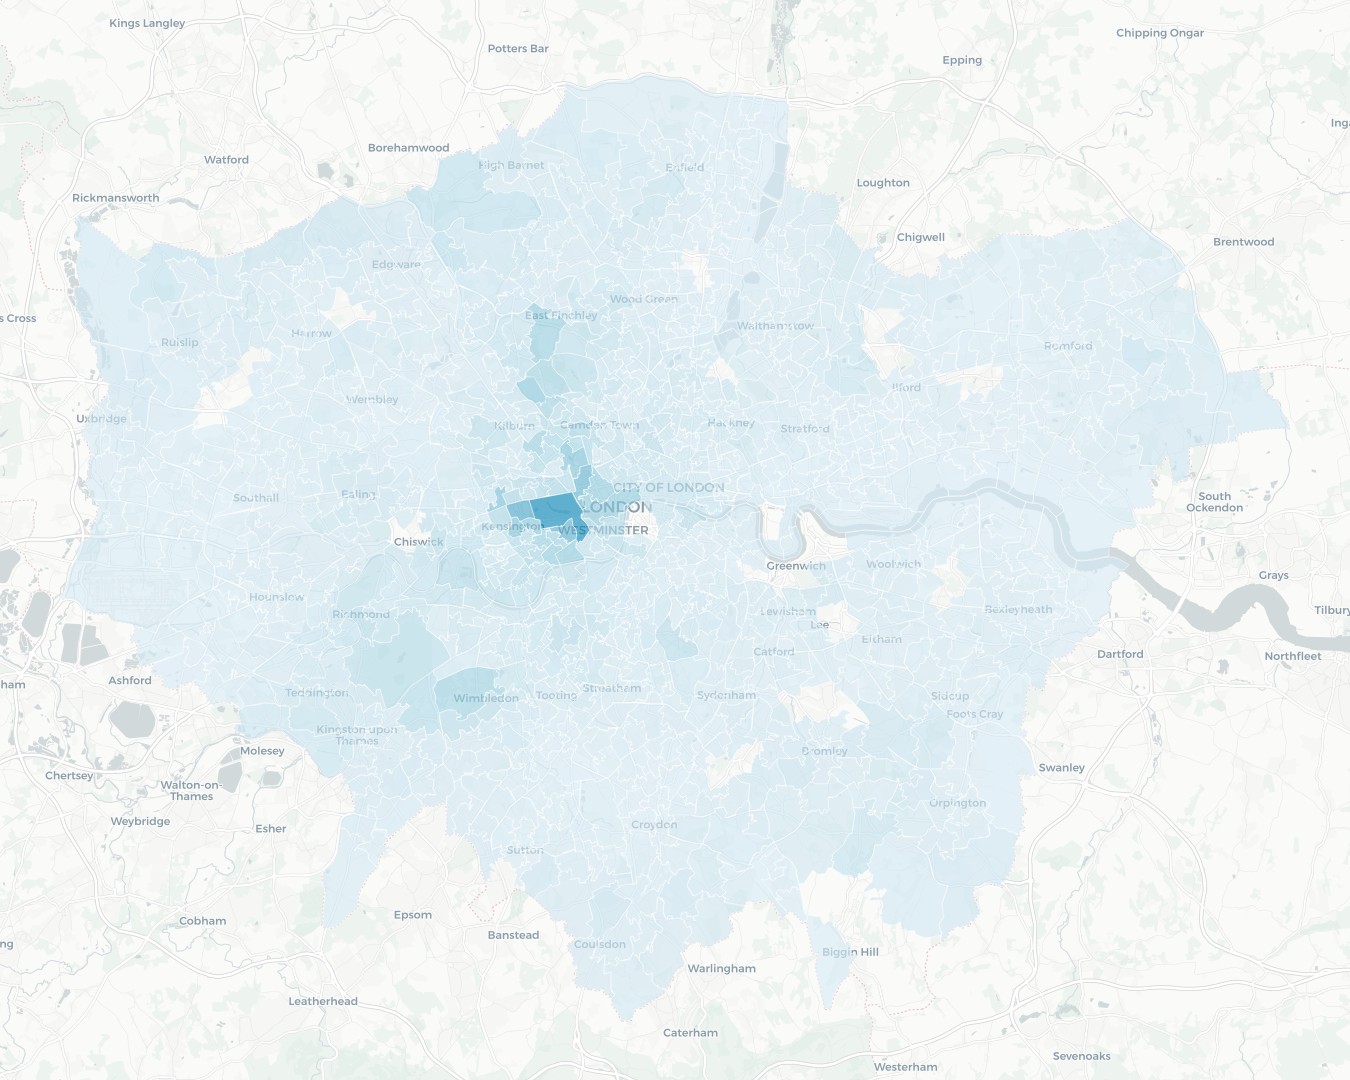
\includegraphics[width=.95\linewidth]{images/housing_raw_mean.png}
      \caption{Mean Housing Price}
      \label{fig:1(a)}
  \end{subfigure}
  \begin{subfigure}{.45\textwidth}
      \centering
      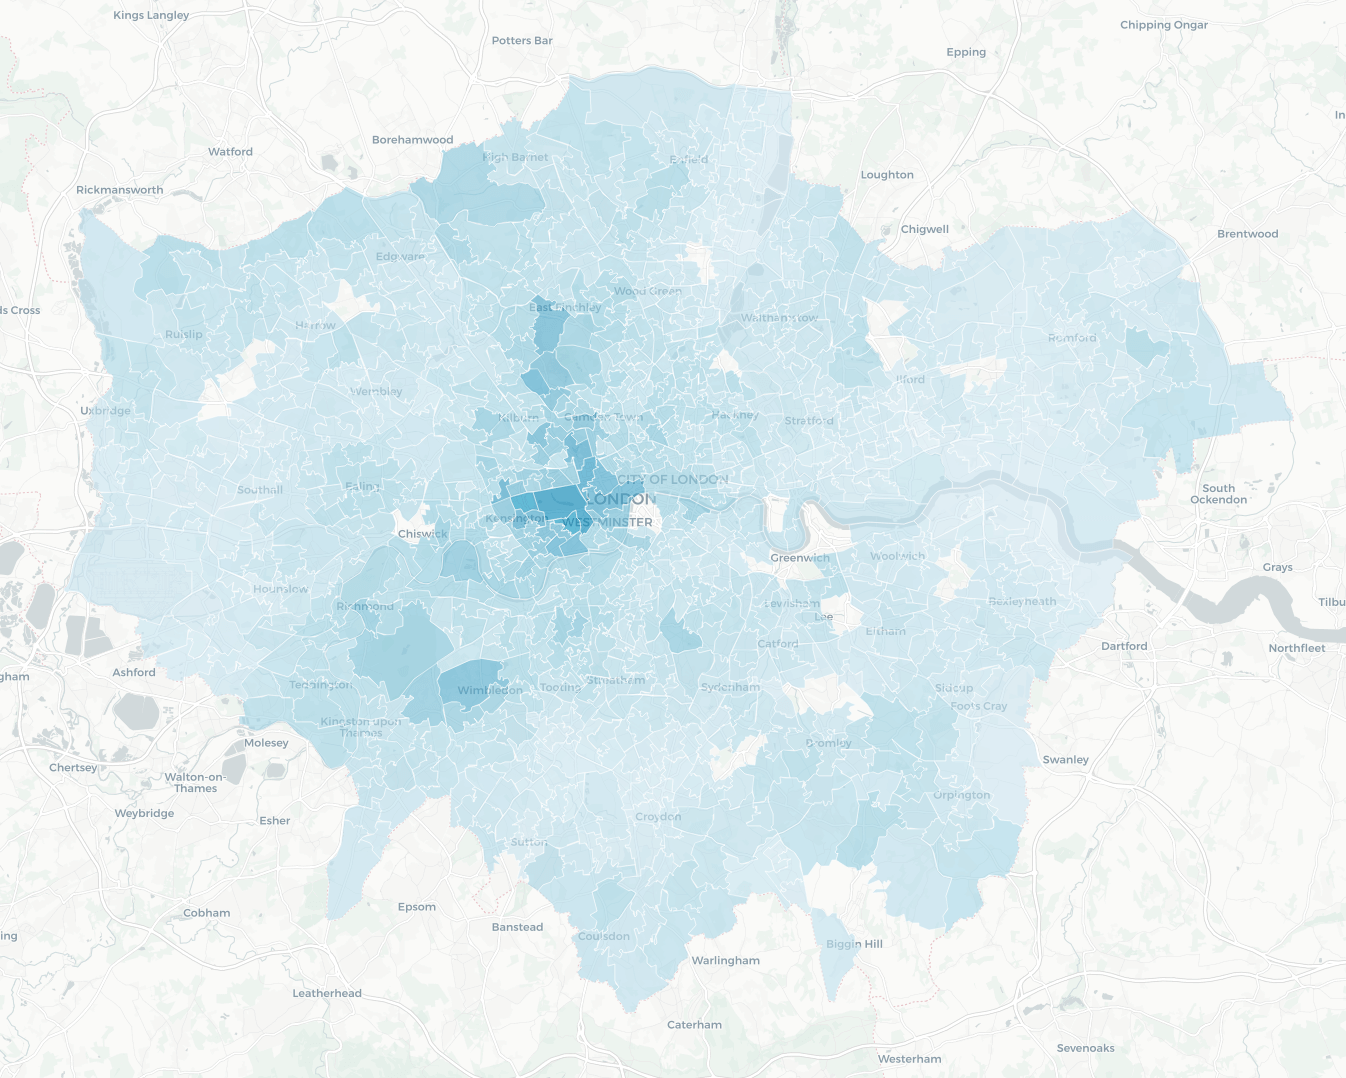
\includegraphics[width=.95\linewidth]{images/housing_log_mean.png}
      \caption{log(Mean Housing Price)}
      \label{fig:1(b)}
  \end{subfigure}
  \caption{Housing price distribution across Greater London}
  \label{fig:price_distribution}
\end{figure}

\subsection{Distance}
london msoa
multipolygons

uber movement data 
pairwise hours 789

\subsection{Geographical Features}
openstreetmap

\subsection{Private School Data}
\texttt{geocoders.Nominatim} module from \texttt{geopy} library in Python is used to convert addresses into longitudes and latitudes.



\section{Variable Construction}
\subsection{Distance Measures}
The following illustrates how two measures of distance are constructed. To ensure an approximately normal distribution, both distance measures are log-transformed in the regression models.
\subsubsection{Orthodromic Distance}
The first measure of distance is the distance between two points on a sphere; the centroid of a given area $C_k$ and the centroid of the CBD, $C_0$, which is then converted to miles for ease of interpretation. Each MSOA is represented by a simple polygon where each vertex consists of longitude and latitude in the standard geographic coordinate system (Bolstad, 2016). Let $v_{i,j}$ be a vertex in a N-gon where $v_i$ is a longitude and $v_j$ is a latitude. Then the centroid for a given a $k$ is expressed as 

\begin{center}
    $C_k = (C_{ki}, C_{kj})  = (\frac{1}{n} \Sigma_{i=1}^{N} v_i, \frac{1}{n} \Sigma_{j=1}^{N} v_j) $
\end{center}

where $C_{ki}$ and $C_{kj}$ are longitude and latitude for the centroid, respectively. Since the centroids are relatively close to each other with each located in our setting, the Haversine formula (Van Brummelen, 2013) is used for numerical stability to calculate the distance between two points on a sphere\footnote{The Haversine formula is computationally better conditioned than the arc length formula when two points are close to each other due to rounding errors}, $C_0$ and $C_k$, such that

\begin{center}
    $d =2 r \arcsin \left(\sqrt{\sin ^{2}\left(\frac{C_{0i}-C_{ki}}{2}\right)+\cos \left(C_{ki}\right) \cos \left(C_{0i}\right) \sin ^{2}\left(\frac{C_{0j}-C_{kj}}{2}\right)}\right)$
\end{center}
where $r$ is the radius of earth in a desired unit of length, which in this case miles with $r = 3956$. 

\subsubsection{Uber Movement Distance}
\subsection{Geographical Features from OpenStreetMap}

\section{Empirical Analysis}
\subsection{Model Specifications}
\subsection{Results}
\subsection{Robustness Checks}

\section{Discussion}
\subsection{Causal Interpretations}
\subsection{External Validity}
\subsection{Limitations and Future Work}

\section{Conclusion}


% \section{Examples of citations, figures, tables, references}
% \label{sec:others}
% \lipsum[8] \cite{kour2014real,kour2014fast} and see \cite{hadash2018estimate}.

% The documentation for \verb+natbib+ may be found at
% \begin{center}
%   \url{http://mirrors.ctan.org/macros/latex/contrib/natbib/natnotes.pdf}
% \end{center}
% Of note is the command \verb+\citet+, which produces citations
% appropriate for use in inline text.  For example,
% \begin{verbatim}
%   \citet{hasselmo} investigated\dots
% \end{verbatim}
% produces
% \begin{quote}
%   Hasselmo, et al.\ (1995) investigated\dots
% \end{quote}

% \begin{center}
%   \url{https://www.ctan.org/pkg/booktabs}
% \end{center}


% \subsection{Figures}
% \lipsum[10] 
% See Figure \ref{fig:fig1}. Here is how you add footnotes. \footnote{Sample of the first footnote.}
% \lipsum[11] 

% \begin{figure}
%   \centering
%   \fbox{\rule[-.5cm]{4cm}{4cm} \rule[-.5cm]{4cm}{0cm}}
%   \caption{Sample figure caption.}
%   \label{fig:fig1}
% \end{figure}

% \subsection{Tables}
% \lipsum[12]
% See awesome Table~\ref{tab:table}.

% \begin{table}
%  \caption{Sample table title}
%   \centering
%   \begin{tabular}{lll}
%     \toprule
%     \multicolumn{2}{c}{Part}                   \\
%     \cmidrule(r){1-2}
%     Name     & Description     & Size ($\mu$m) \\
%     \midrule
%     Dendrite & Input terminal  & $\sim$100     \\
%     Axon     & Output terminal & $\sim$10      \\
%     Soma     & Cell body       & up to $10^6$  \\
%     \bottomrule
%   \end{tabular}
%   \label{tab:table}
% \end{table}

% \subsection{Lists}
% \begin{itemize}
% \item Lorem ipsum dolor sit amet
% \item consectetur adipiscing elit. 
% \item Aliquam dignissim blandit est, in dictum tortor gravida eget. In ac rutrum magna.
% \end{itemize}


\bibliographystyle{unsrt}  
%\bibliography{references}  %%% Remove comment to use the external .bib file (using bibtex).
%%% and comment out the ``thebibliography'' section.


%%% Comment out this section when you \bibliography{references} is enabled.
\newpage
\begin{thebibliography}{1}

\bibitem{kour2014real}
George Kour and Raid Saabne.
\newblock Real-time segmentation of on-line handwritten arabic script.
\newblock In {\em Frontiers in Handwriting Recognition (ICFHR), 2014 14th
  International Conference on}, pages 417--422. IEEE, 2014.

\bibitem{kour2014fast}
George Kour and Raid Saabne.
\newblock Fast classification of handwritten on-line arabic characters.
\newblock In {\em Soft Computing and Pattern Recognition (SoCPaR), 2014 6th
  International Conference of}, pages 312--318. IEEE, 2014.

\bibitem{hadash2018estimate}
Guy Hadash, Einat Kermany, Boaz Carmeli, Ofer Lavi, George Kour, and Alon
  Jacovi.
\newblock Estimate and replace: A novel approach to integrating deep neural
  networks with existing applications.
\newblock {\em arXiv preprint arXiv:1804.09028}, 2018.

\end{thebibliography}

\end{document}
